% ---
% Arquivo com a Introdução do Trabalho de Conclusão de Curso do aluno
% Daniel Noriaki Kurosawa
% da Escola Politécnica da Universidade de São Paulo
% ---

	\chapter{Introdução} 
	\addcontentsline{toc}{chapter}{Introdução}
	Hoje, através do uso de tecnologias de telecomunicação, é possível a transmissão de grandes volumes de informações a ambientes remotos sem a necessidade da presença física das partes envolvidas, tornando a interação prática, rápida e fisicamente segura.\par
	
	 Existem casos porém\cite{uses-arm}\cite{uses-robot}, em que a interação física a distância com um ambiente remoto é necessária devido a periculosidade ou a dificuldades de acesso ao mesmo, que trariam riscos a um ser humano. Para tais tipo de tarefa, cada vez mais há a substituição de seres humanos por máquinas específicas tais como braços robóticos \par
	
	%Braços robóticos possuem uma ampla gama de aplicações,substituindo seres humanos em tarefas em locais de difícil acesso, repetitivas, ou de alta periculosidade, indo seu uso desde o desarmamento de bombas ao uso em missões espaciais\cite{uses-arm}, passando por processos industriais\cite{uses-robot}.\par
	
	 Porém, apesar do aumento na segurança para o usuário, muitas das abordagens para a operação de um braço robótico continuam complexas e anti-intuitivas  necessitando do uso de artifícios como controles remotos\cite{datasheet-caliber} e joysticks\cite{joystick}. \par
	 
	 Uma segunda linha de pensamento tenta se aproveitar de semelhanças físicas entre o corpo humano e o braço robótico e faz uso, por exemplo, de sensores \cite{wearable} e marcadores\cite{tracker-based} presos ao corpo. Entretanto, essas abordagens podem se provar incomodas ou restritivas em relação à movimentação do usuário devido por exemplo, a ocultação de um marcador ou a rigidez de um sensor vestível.\cite{kinect-based}\par 
	 
	 Uma solução para essas restrições, estudada neste trabalho é o uso de tecnologia de rastreamento visual sem marcadores, que permite que o usuário não mais se preocupe com as restrições de movimento impostas, tornando o controle mais natural.\cite{kinect-based} \par 
	
	 Muitas vezes também, para a operação remota de tais equipamentos, é necessária a transmissão de imagens do ambiente remoto.\par
	 Este trabalho estuda o uso de um sistema de imersão visual através do uso de um óculos realidade virtual por rastreamento dos movimentos da cabeça do usuário e um sistema de câmeras estereoscópicas ao projeto, com a finalidade de criar uma experiência imersiva ao usuário.\par 
	
	 
	
	
	
	
	\begin{figure}[ht!]
		\caption{\label{fig_diagrama}Diagrama do projeto}
		\begin{center}
		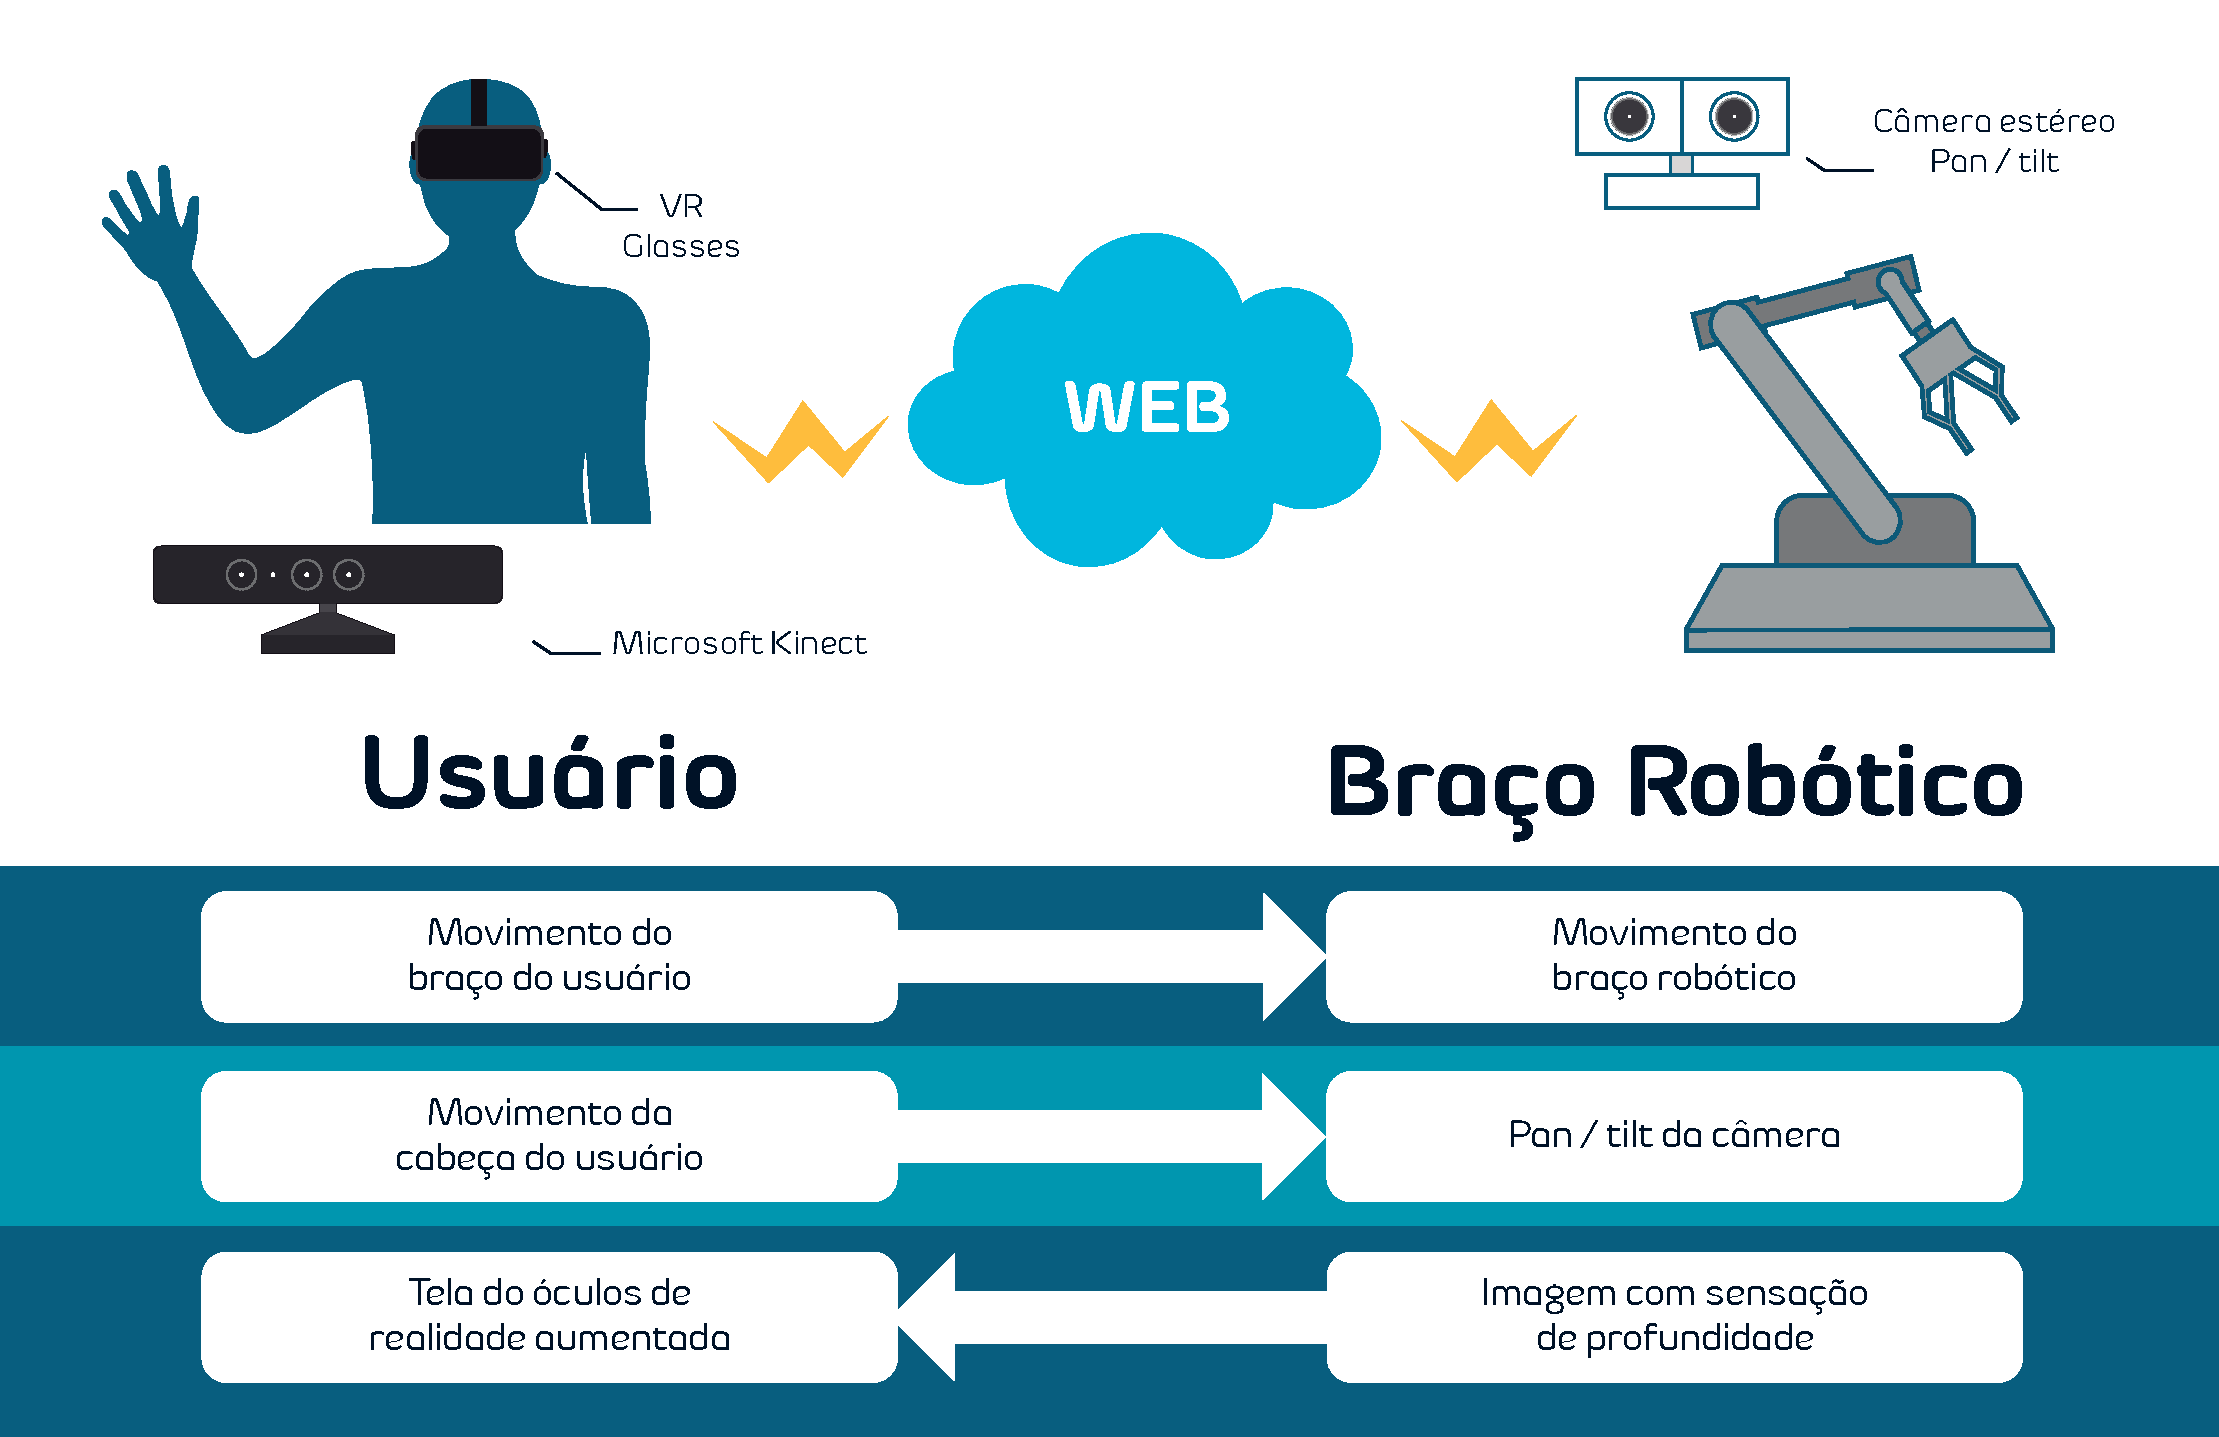
\includegraphics[width=\textwidth]{projectchart.pdf}	
		\end{center}
		\legend{Fonte: Autor}
	\end{figure}
	

	
	\section{Motivação}\label{sec-motivacao}
	

	
	Este projeto surge da ideia de tentar unir conceitos de engenharia de automação, ênfase da graduação do autor, a conceitos engenharia de computação, área de pesquisa do professor orientador do projeto.
	
	Dentro deste contexto multidisciplinar, naturalmente a ideia de um projeto de Internet of Things surge, sendo então discutidas ideias sobre possíveis tema para estudo. Entre as alternativas estudadas, experiências do Jet Propulsion Laboratory da NASA\cite{nasa-project} surgem como motivação para este trabalho.
	 

		\section{Ideias iniciais e alternativas do projeto}\label{subsec-iniciais}
	
	Inicialmente, a pesquisa inicial tratou os seguintes temas:\par
	
	
	\begin{itemize}[noitemsep]
		\item Geração de trajetória para braço robótico usando Microsoft Kinect;
		\item Captura de movimentos usando giroscópio;
		\item Algoritmos anti-drifting de giroscópio;
		\item Captura de imagens estereoscópicas em tempo real;
		\item Arduino;
		\item Raspberry Pi;
		\item Particle Photon;
		\item Internet of Things;
	\end{itemize}
	As ideias iniciais continham premissas que envolviam o uso de redes neurais para o controle do braço mecânico, utilizando um controlador ANFIS-PID para o controle dos motores, chegando a ser testado.\par
	Posteriormente, em virtude de limitações de memória do hardware e a complexidade adicionada ao projeto, os algoritmos de redes neurais foram excluídos do escopo do projeto.
	O formato final é tratado na seção seguinte(\autoref{sec-objetivo}).
	\section{Objetivo}\label{sec-objetivo}

	Este estudo propõe um  sistema de imersão e interação do usuário em um ambiente remoto através da  operação de um braço mecânico e do uso de um sistema de imersão visual.\par

	A face de interação do projeto é representada pela operação de um braço robótico à distância, realizada através do uso do sensor de captura de movimento Microsoft Kinect e de um braço robótico conectado a uma rede WiFi.\par
	
	O segundo objetivo do projeto trata da imersão visual do usuário no ambiente remoto
	em que ocorre a interação. Tal imersão será realizada através de um sistema de câmeras estereoscópicas com motores de rotação pan/tilt, uso de óculos de realidade virtual para a recepção das imagens das câmeras e rastreamento de movimentos da cabeça do usuário para o controle de movimentação dos motores.\par
		
	Visando uma maior adaptabilidade de suas partes a outras aplicações, o projeto será encarado de forma modular, de forma que as partes componentes descritas acima poderão ser utilizadas independentemente.\par
	
	 Além disso, o rigor metodológico é uma das preocupações centrais deste trabalho, o que inclui um refinamento na maneira de definir os requisitos do sistema, representado pelo RM-ODP.
	